\section{Scalogram}

The scolargrams show the time frequency analysis content of the data for each region. Frequencies of higher magnitude will show up with brighter colors, which can also be seen on the magnitude colorbar for comparison of the magnitude in values.. 
The freqency of the scalograms vary from 2.7370 Hz to 0.0031 Hz. This means according to the litteraturethat bands of cardiac, respiratory, endothelial, myogenic and neurogenic is represented in the wavelet frequency span for the time frequency analysis. [citation]
The wavelet is shown before and after correction of the signal. 

The scalogram in \figref{fig:uncuffed_sub3_roi8_corr} is representing the wavelet transformation of the raw signal without the correction. It is clear to see the frequency from the noise in the signal. 

The noise components:
\begin{itemize}
	\item White noise
	\item Drift between each interval
	\item Jumps
	\item Generel drift in the signal
\end{itemize}

The four noise components is disturbing the signal to make the cwt analysis valid because the noise is not constant in each recording.....
....
After the drift correction is added to the signal, the energy  has been reduced at this area induced from the jump. With this correction it should be more accurate to use the data for the statistics because. The signal should still be  preserved. 

\begin{figure}[H]
	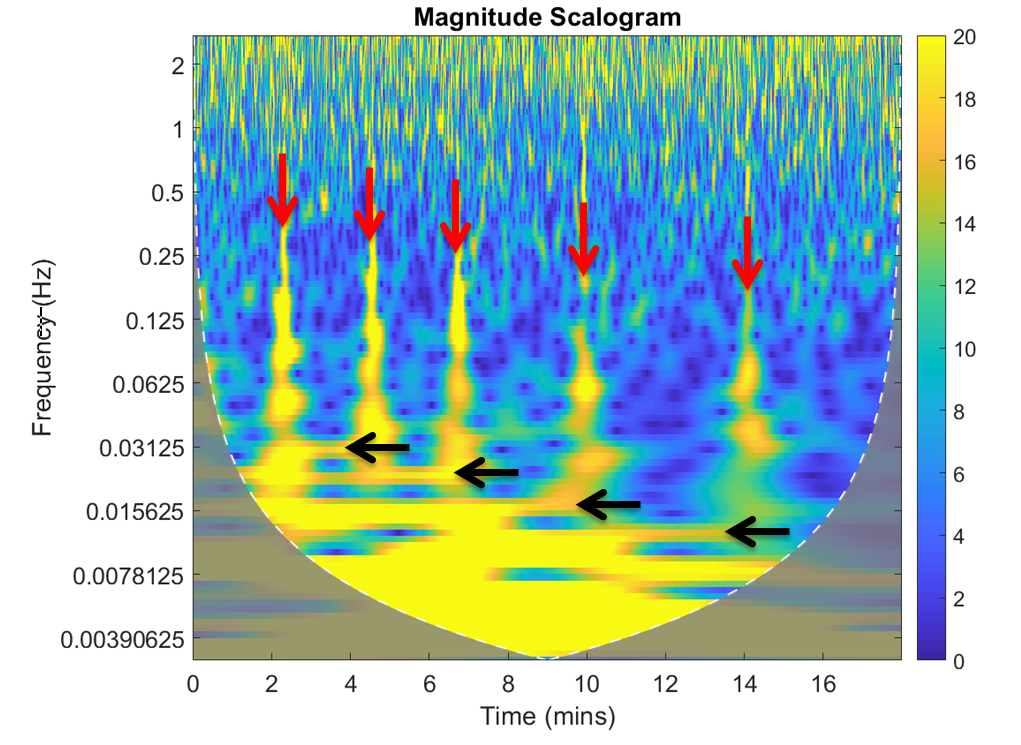
\includegraphics[width=0.7\textwidth]{figures/uncuffed_sub3_roi8_uncorr}
	\caption{Scalogram from the original data of region 15 in the uncuffed recording of subject 1, where high spike magnitudes can be seen induced by the jumps.}
	\label{fig:scalogram_uncorr}
\end{figure}




\begin{figure}[H]
	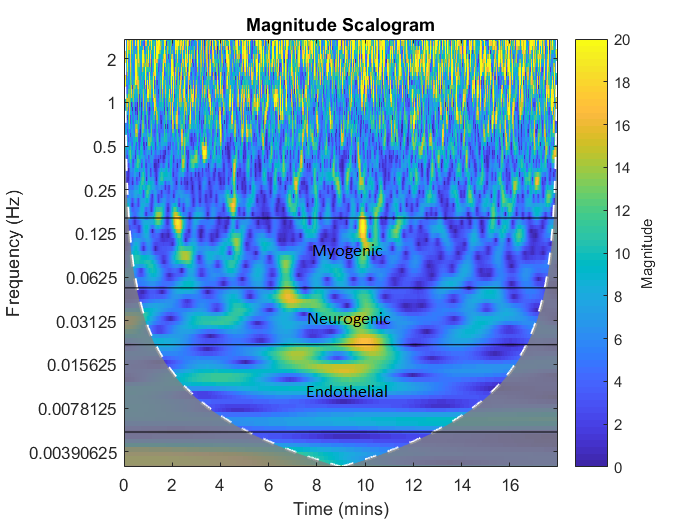
\includegraphics[width=1\textwidth]{figures/uncuffed_sub3_roi8_corr}
	\caption{Scalogram from the corrected data of region 24 in the cuffed recording of subject 1, where a dampening of the high spike and drift magnitudes induced by the jumps has been achieved.}
	\label{fig:scalogram_corr}
\end{figure} 